\section{Canadian Grand prix}

\subsection{Circuit Analysis}

\textbf{Circuit Name:} Circuit Gilles-Villeneuve (Montréal, Canada) \\
\textbf{Length:} 4.361 km - \textbf{Laps:} 70 - \textbf{Total Distance:} 305.270 km

\begin{figure}[H]
    \centering
    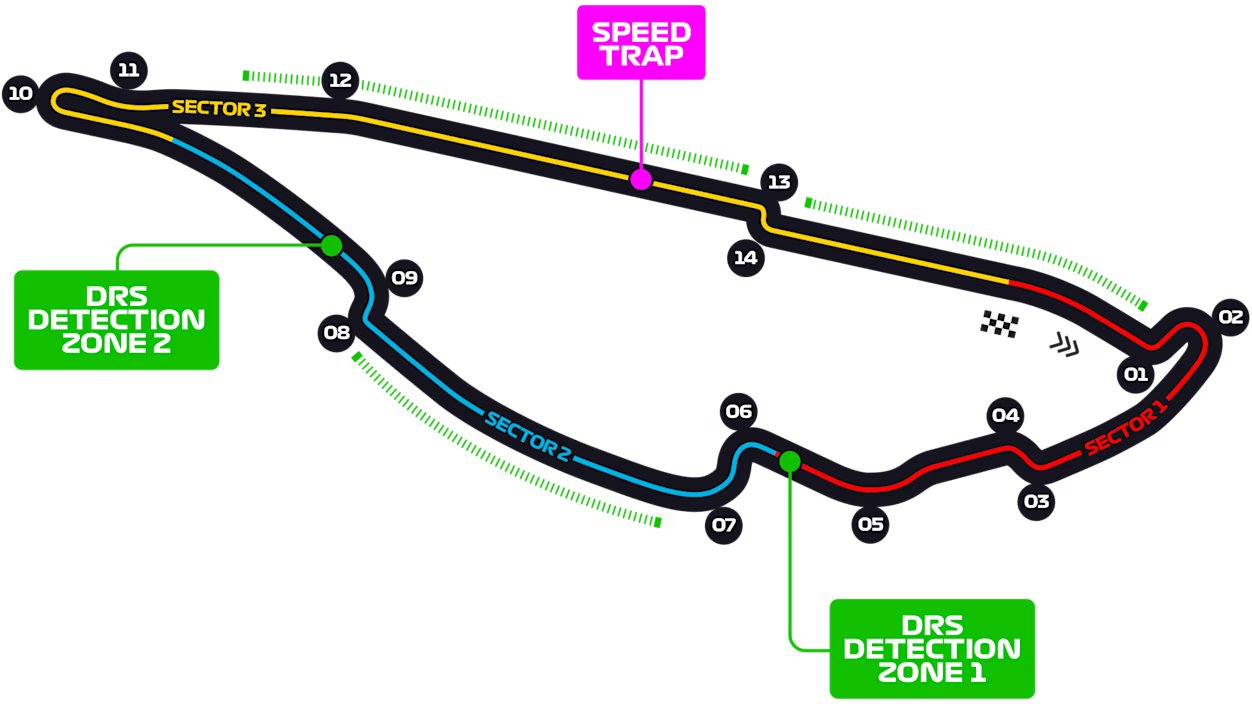
\includegraphics[width=0.75\linewidth]{images/9.Canada_Circuit.jpg}
\end{figure}

\begin{itemize}
    \item \textbf{Lap Record} : 1:10.240 (2019, Sebastian Vettel – Ferrari).
    
    \item \textbf{Number of Corners \& Key Features} : 13 turns (8 right, 5 left) - Semi-permanent circuit on Notre Dame Island. Famous for the “Wall of Champions” at the final chicane. Mix of long straights and heavy braking chicanes, rewarding top speed and strong traction.
    
    \item \textbf{Braking Zones \& Traction} : Heavy braking into Turns 1, 10 (L’Epingle hairpin), and the final chicane. Traction is crucial out of Turn 10 onto the long Casino Straight.
    
    \item \textbf{DRS \& Overtaking} : Three DRS zones (start/finish straight, Casino Straight, between Turns 7–8). \\
    Prime overtaking spots at the hairpin (T10) and into the final chicane.
    
    \item \textbf{Tyre Degradation \& Strategy} : Tyre degradation usually low, but graining possible in cool or damp conditions. \\
    One-stop strategies possible, though Safety Cars often change plans.
    
    \item \textbf{Weather \& Environment} : Early summer weather is unpredictable, frequent risk of rain. \\
    Cooler temps increase risk of graining. \\
    Safety Car probability high due to walls and narrow runoff.
\end{itemize}

\textbf{Strategic Summary :}
Montréal rewards power units, braking stability, and traction. Track position is important but overtaking is more feasible than Monaco or Imola. Strategy must remain flexible due to high chance of Safety Car or weather disruption.


\subsection{Race Analysis}

\textbf{Date:} 9 June 2024 — 14:00 local time 

\begin{itemize}
    \item \textbf{Qualifying Summary} : \textbf{Pole Position:} George Russell (Mercedes) – 1:12.000 - (equal to Verstappen, Russell ahead by setting time first). \\
    Grid: Verstappen 2nd, Norris 3rd, Piastri 4th.\\
    Leclerc and Sainz started from the midfield after poor qualifying.
    
    \item \textbf{Race Summary} : \textbf{Winner:} Max Verstappen (Red Bull).\\
    \textbf{Podium:} 1. Verstappen - 2. Norris - 3. Russell.\\
    \textbf{Technical issues:} Leclerc (power unit).\\
    \textbf{Notable incidents:} Multiple Safety Cars — including one on lap 54 after Sainz’s crash at Turn 6.
    
    \item \textbf{Strategies} : Most teams switched between slicks and intermediates.\\
    - Verstappen timed pit stops perfectly (under Safety Car), maintaining track position.\\ 
    - Norris lost victory chance due to unlucky Safety Car timing. 
    - Mercedes split strategies, Russell and Hamilton both strong on mediums late. 
    Alpine executed perfectly, double points finish from deep in the grid.
    
    \item \textbf{Performance Trends} : \textbf{Red Bull:} proved adaptable in mixed weather, Verstappen perfect under pressure.
    \textbf{McLaren:} Norris fastest in race conditions, unlucky with SC. Piastri competitive but edged by Mercedes. 
    \textbf{Mercedes:} Best weekend of 2024 so far, Russell pole + podium, Hamilton fastest lap and P4. 
    \textbf{Ferrari:} Disaster: poor quali, Leclerc PU failure, Sainz crash. Big blow in championship. 
    \textbf{Aston Martin:} Strong, Alonso P6, Stroll P7 at home GP. 
    \textbf{Racing Bulls:} Ricciardo excellent (Qualified P5, P8 despite penalty), Tsunoda error-strewn (P14). 
    \textbf{Alpine:} Best weekend so far, Gasly P9, Ocon P10, both in points. 
    \textbf{Haas:} Great opening laps on wets, but faded to P11–12.
    
    \item \textbf{Championship Impact} : \textbf{Drivers:} Verstappen 194 points, Leclerc 138, Norris 131.\\
    \textbf{Constructors:} Red Bull 301, Ferrari 252, McLaren 212, Mercedes 124.    
\end{itemize}

\textbf{Key Takeaway :}
Verstappen thrived in chaos, securing another win in a rain-affected race. McLaren continued their strong momentum, while Mercedes finally showed flashes of competitiveness. Ferrari’s double DNF dealt a huge blow to their title hopes.


\subsection{Link \& Takeaway}

\begin{itemize}
    \item The high Safety Car probability at Montréal struck again, timing was decisive, costing Norris and saving Verstappen. 
    \item Ferrari’s failure exposed their fragility: from consistency to a double DNF. 
    \item Mercedes took a genuine step forward, showing both one-lap and race pace. 
    \item McLaren confirmed they are now Red Bull’s closest rivals. 
    \item Alpine finally delivered a clean weekend and double points. 
    \item Aston Martin secured much-needed points with both drivers, stabilising their season. 
\end{itemize}